\documentclass{homework}
\newcommand{\R}{\textbf{R}}
\newcommand{\dee}{\;\text{d}}
\newcommand{\eps}{\varepsilon}
\newcommand{\pl}[2]{\frac{\partial #1}{\partial #2}}
\newcommand{\dl}[2]{\frac{\text{d} #1}{\text{d} #2}}
\newcommand{\sgn}{\text{sgn}}
\newcommand{\bigoh}{\mathcal{O}}
\usepackage{enumitem}

\newcommand{\hwclass}{Math 6108}
\newcommand{\hwname}{Jacob Hauck}
\newcommand{\hwtype}{Homework}


\usepackage{listings}
\usepackage{booktabs}

\newcommand{\hwnum}{4}
\renewcommand{\questiontype}{Problem}

\begin{document}
	\maketitle
	
	\question
	Consider
	\begin{equation}
		\label{eq:ode}
		y' = \left(1-2t^3\right)y^2, \quad t > 0; \qquad y(0) = 1.
	\end{equation}
	
	\begin{alphaparts}
		\questionpart In order to apply the second-order Taylor series method, we need to use the ODE (\ref{eq:ode}) to find $y''$ in terms of $y$:
		\begin{equation*}
			y'' = \dl{}{t}\big[\left(1-2t^3\right)y^2\big] = -6t^2y^2 + 2\left(1-2t^3\right)yy' = -6t^2y^2 + 2\left(1-2t^3\right)^2y^3.
		\end{equation*}
		Then the second-order Taylor series method is given by
		\begin{equation*}
			\begin{cases}
				y^{n+1} = y^n + k\left(1-2t_n^3\right)\left(y^n\right)^2 + \frac{k^2}{2}\left[-6t_n^2\left(y^n\right)^2 + 2\left(1-2t_n^3\right)^2\left(y^n\right)^3\right], & n = 0,1,2,\dots \\
				y^0 = 1.
			\end{cases}
		\end{equation*}
		This method is implemented in \verb*|ts2.m|.
		
		\questionpart The recursive rule for the two-step Adams-Bashforth method is given by 
		\begin{equation*}
			y^{n+1} = y^n + k\left[\frac{3}{2}f\left(t_n, y^n\right) - \frac{1}{2}f\left(t_{n-1}, y^{n-1}\right)\right], \quad n \ge 0,
		\end{equation*}
		where, in our case, $f(t,y) = \left(1-2t^3\right)y^2$. We use the forward Euler method to obtain $y^1$, as the forward Euler method has second-order local truncation error. Thus, our scheme is
		\begin{equation*}
			\begin{cases}
				y^{n+1} = y^n + k\left[\frac{3}{2}\left(1-2t_n^3\right)\left(y^n\right)^2 - \frac{1}{2}\left(1-2t_{n-1}^3\right)\left(y^{n-1}\right)^2\right] & n = 1, 2, 3,\dots \\
				y^1 = y^0 + k\left(1-2t_0^3\right)\left(y^0\right)^2 \\
				y^0 = 1.
			\end{cases}
		\end{equation*}
		This method is implemented in \verb*|ab2.m|.
		
		\questionpart The recursive rule for the trapezoidal method is given by
		\begin{equation*}
			y^{n+1} = y^n + k\left[\frac{1}{2}f\left(t_n, y^n\right) + \frac{1}{2}f\left(t_{n+1}, y^{n+1}\right)\right],\quad n \ge 0,
		\end{equation*}
		where, in our case, $f(t,y) = \left(1-2t^3\right)y^2$. Then our scheme is given implicitly by
		\begin{equation*}
			\begin{cases}
				y^{n+1} = y^n + \frac{k}{2}\left[\left(1-2t_n^3\right)\left(y^n\right)^2 + \left(1-2t_{n+1}^3\right)\left(y^{n+1}\right)^2\right] & n = 0,1,2,\dots \\
				y^0 = 1.
			\end{cases}
		\end{equation*}
		In order to solve the implicit equation for $y^{n+1}$, we can equivalently use Newton's method to find the root of
		\begin{equation*}
			f_n(y) = y - y^n - \frac{k}{2}\left[\left(1-2t_n^3\right)\left(y^n\right)^2 + \left(1-2t_{n+1}^3\right)y^2\right], \quad n = 0,1,2,\dots
		\end{equation*}
		We will need $f_n'$ to use Newton's method:
		\begin{equation*}
			f_n'(y) = 1- k(1-2t_{n+1}^3)y.
		\end{equation*}
		This method is implemented in \verb*|tp.m| and uses the implementation of Newton's method in \verb*|newton.m|.
		
		\questionpart The recursive rule for the midpoint method is given by
		\begin{equation*}
			y^{n+1} = y^n + kf\left(t_n + \frac{k}{2}, \frac{y^n + y^{n+1}}{2}\right), \quad n \ge 0,
		\end{equation*}
		where, in our case, $f(t,y) = \left(1-2t^3\right)y^2$. Then our scheme is given implicitly by
		\begin{equation*}
			\begin{cases}
				y^{n+1} = y^n + k\left(1-2\left(t_n + \frac{k}{2}\right)^3\right)\left(\frac{y^n + y^{n+1}}{2}\right)^2 & N = 0,1,2,\dots\\
				y^0 = 1.
			\end{cases}
		\end{equation*}
		To solve the implicit equation for $y^{n+1}$, we can equivalently use Newton's method to find the root of
		\begin{equation*}
			f_n(y) = y - y^n - k\left(1-2\left(t_n + \frac{k}{2}\right)^3\right)\left(\frac{y^n + y}{2}\right)^2, \quad n = 0,1,2,\dots
		\end{equation*}
		To use Newton's method, we need $f_n'$:
		\begin{equation*}
			f_n'(y) = 1 - \frac{k}{2}\left(1-2\left(t_n + \frac{k}{2}\right)^3\right)(y^n + y).
		\end{equation*}
		This method is implemented in \verb*|mp.m| and uses the implementation of Newton's method in \verb*|newton.m|.
		
		\questionpart To compare the above methods with the exact solution of (\ref{eq:ode}), we first need to determine the exact solution. Using separation of variables, we have
		\begin{equation*}
			\frac{y'}{y^2} = 1-2t^3 \implies -y^{-1} = t - \frac{t^4}{2} + C, \quad \text{some C $\in \R$}.
		\end{equation*}
		Since $y(0)=1$, it follows that $C = -1$, so
		\begin{equation*}
			y(t) = \frac{1}{\frac{t^4}{2} - t + 1}
		\end{equation*}
		is the exact solution of the (\ref{eq:ode}).
		
		Using the code in \verb*|problem1_calculations.m|, we run the above four methods with various step sizes and compute the error at $t = 2$. The results can be found in \verb*|p1_output.txt| and are summarized in Table \ref{table:errors}.
		\begin{table}[h]
			\centering
			\begin{tabular}{@{}lllllllll@{}}
				\toprule
				& \multicolumn{2}{c}{TS2} & \multicolumn{2}{c}{TP} & \multicolumn{2}{c}{AB2} & \multicolumn{2}{c}{MP} \\
				\cmidrule(lr){2-3}
				\cmidrule(lr){4-5}
				\cmidrule(lr){6-7}
				\cmidrule(lr){8-9}
				$k$ & Error & Rate & Error & Rate & Error & Rate & Error & Rate \\
				\midrule
				1/4 & 2.3989e-03 & - & 6.2704e-03 & - & 1.8370 & - & 1.1923e-02 & - \\
				1/8 & 4.3209e-03 & -0.8489 & 1.4774e-03 & 2.0854 & 6.9392e-03 & 8.0483 & 2.9800e-03 & 2.0004 \\
				1/16 & 8.8105e-04 & 2.2940 & 3.6416e-04 & 2.0204 & 1.8133e-03 & 1.9361 & 7.4426e-04 & 2.0014 \\
				1/32 & 1.9901e-04 & 2.1463 & 9.0720e-05 & 2.0050 & 4.4886e-04 & 2.0142 & 1.8601e-04 & 2.0004 \\
				1/64 & 4.7427e-05 & 2.0691 & 2.2660e-05 & 2.0012 & 1.1053e-04 & 2.0217 & 4.6499e-05 & 2.0001 \\
				1/128 & 1.1585e-05 & 2.0333 & 5.6638e-06 & 2.0003 & 2.7368e-05 & 2.0139 & 1.1624e-05 & 2.0000 \\
				1/256 & 2.8636e-06 & 2.0163 & 1.4158e-06 & 2.0000 & 6.8058e-06 & 2.0076 & 2.9061e-06 & 2.0000 \\
				\bottomrule
			\end{tabular}
			\caption{Numerical errors and convergence rates at $t=2$}
			\label{table:errors}
		\end{table}
		
		\questionpart The code to plot the errors in Table \ref{table:errors} on a log-log plot can be found in \verb*|problem1_calculations.m|. The resulting plot is given in Figure \ref{fig:error_plot}.
		\begin{figure}[h]
			\centering
			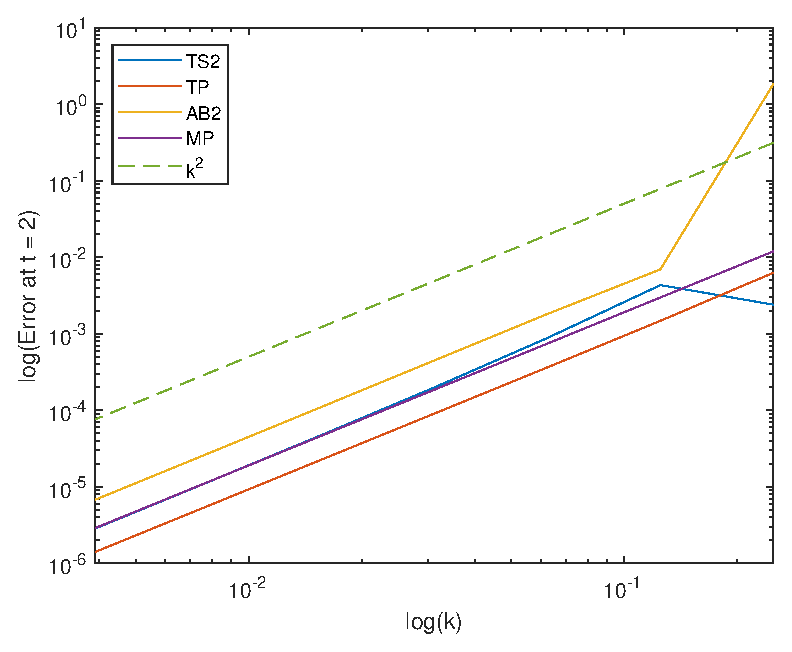
\includegraphics{p1f_plot.eps}
			\caption{Numerical errors at $t = 2$ versus time step}
			\label{fig:error_plot}
		\end{figure}
		
		\textbf{Observations}
		\begin{itemize}
			\item By comparison with the reference line $k^2$, we see that all four methods have second-order error, which agrees with the theoretical predictions we had for these methods.
			\item For the largest step size, there is a significant deviation in the error trend for the second-order Taylor series (TS2) and two-step Adams-Bashforth (AB2) methods. This may be due to the fact that these methods are explicit and less stable than the implicit midpoint (MP) and trapezoidal (TP) methods.
		\end{itemize}
	\end{alphaparts}
	
	\question
	
	\textbf{Adams-Bashforth}
	
	One step of the three-step Adams-Bashforth method is given by
	\begin{equation*}
		y^{n+3} = y^{n+2} + k\left(b_2f(t_{n+2}, y^{n+2}) + b_1f(t_{n+1}, y^{n+1}) + b_0f(t_n, y^n)\right),
	\end{equation*}
	where $b_0$, $b_1$, and $b_2$ are chosen to minimize the order of the local truncation error. Hence, we can find these values by calculating the local truncation error and minimizing its order. Assume that $y^n = y(t_n)$, $y^{n+1} = y(t_{n+1})$, and $y^{n+2} = y(t_{n+2})$. Then the local truncation error is given by
	\begin{equation*}
		y^{n+3} - y(t_{n+3}) = y(t_{n+2}) + k\left(b_2y'(t_{n+2}) + b_1y'(t_{n+1}) + b_0y'(t_n)\right) - y(t_{n+3}).
	\end{equation*}
	Using Taylor expansion about $t_n$ gives
	\begin{alignat*}{2}
		y^{n+3} - y(t_{n+3}) &={}&  &y(t_n) + 2ky'(t_n) + \frac{4k^2}{2}y''(t_n) + \frac{8k^3}{6}y'''(t_n) + \bigoh(k^4) \\
		&& & + kb_2y'(t_n) + 2k^2b_2y''(t_n) + \frac{4k^3}{2}b_2y'''(t_n) + \bigoh(k^4) \\
		&&& + b_1ky'(t_n) + b_1k^2y''(t_n) + \frac{k^3}{2}b_1y'''(t_n) + \bigoh(k^4) \\
		&&& + b_0ky'(t_n) - y(t_n) - 3ky'(t_n) - \frac{9k^2}{2}y''(t_n) - \frac{27k^3}{6}y'''(t_n) + \bigoh(k^4) \\
		&={}&& (b_2 + b_1 + b_0 - 1)ky'(t_n) + \left(2b_2 + b_1 - \frac{5}{2}\right)k^2y''(t_n) + \left(2b_2+\frac{1}{2}b_1-\frac{19}{6}\right)k^3y'''(t_n) + \bigoh(k^4).
	\end{alignat*}
	Thus, the minimum possible order of the local truncation error is 4, which occurs only if
	\begin{align*}
		b_0 + b_1 + b_2 &= 1 \\
		2b_2 + b_1 &= \frac{5}{2} \\
		2b_2 + \frac{1}{2}b_1 &= \frac{19}{6}.
	\end{align*}
	Solving the last two equations for $b_1$ and $b_2$ gives $b_1 = -\frac{4}{3}$, and $b_2 = \frac{23}{12}$. Substituting into the first equations gives $b_0 = \frac{5}{12}$. Therefore, the three-step Adams-Bashforth method is
	\begin{equation*}
		y^{n+3} = y^{n+2} + \frac{k}{12}\left(23f(t_{n+2}, y^{n+2}) - 16f(t_{n+1}, y^{n+1}) + 5f(t_n,y^n)\right).
	\end{equation*}
	
	\textbf{Adams-Moulton}
	
	One step of the three-step Adams-Moulton method is given by
	\begin{equation*}
		y^{n+3} = y^{n+2} + k\left(b_3f(t_{n+3}, y^{n+3}) + b_2f(t_{n+2}, y^{n+2}) + b_1f(t_{n+1}, y^{n+1}) + b_0f(t_n, y^n)\right),
	\end{equation*}
	where $b_0$, $b_1$, $b_2$, and $b_3$ are chosen to minimize the order of the local truncation error.  Hence, we can find these values by calculating the local truncation error and minimizing its order. Assume that $y^n = y(t_n)$, $y^{n+1} = y(t_{n+1})$, and $y^{n+2} = y(t_{n+2})$. Then the local truncation error is given by
	\begin{equation*}
		y^{n+3} - y(t_{n+3}) = y(t_{n+2}) + k\left(b_3f(t_{n+3}, y^{n+3}) + b_2y'(t_{n+2}) + b_1y'(t_{n+1}) + b_0y'(t_n)\right) - y(t_{n+3}).
	\end{equation*}
	Using Taylor expansion about $t_n$ gives
	\begin{alignat*}{2}
		y^{n+3} - y(t_{n+3}) &={}&  &y(t_n) + 2ky'(t_n) + \frac{4k^2}{2}y''(t_n) + \frac{8k^3}{6}y'''(t_n) + \frac{16k^4}{24}y''''(t_n) + \bigoh(k^5) \\
		&&& + kb_3\left(f(t_{n+3}, y^{n+3}) - f(t_{n+3}, y(t_{n+3}))\right) \\
		&&& + kb_3y'(t_n) + 3k^2b_3y''(t_n) + \frac{9k^3}{2}b_3y'''(t_n) + \frac{27k^4}{6}b_3y''''(t_n) + \bigoh(k^5) \\
		&&& + kb_2y'(t_n) + 2k^2b_2y''(t_n) + \frac{4k^3}{2}b_2y'''(t_n) + \frac{8k^4}{6}b_2y''''(t_n) + \bigoh(k^5) \\
		&&& + b_1ky'(t_n) + b_1k^2y''(t_n) + \frac{k^3}{2}b_1y'''(t_n) + \frac{k^4}{6}b_1y''''(t_n) + \bigoh(k^5) \\
		&&& + b_0ky'(t_n) - y(t_n) - 3ky'(t_n) - \frac{9k^2}{2}y''(t_n) - \frac{27k^3}{6}y'''(t_n) - \frac{81k^4}{24}y''''(t_n) + \bigoh(k^5) \\
		&={}&&  kb_3\left(f(t_{n+3}, y^{n+3}) - f(t_{n+3}, y(t_{n+3}))\right) \\
		&&& + (b_3 + b_2 + b_1 + b_0 - 1)ky'(t_n) \\
		&&& + \left(3b_3 + 2b_2 + b_1 -\frac{5}{2}\right)k^2y''(t_n) \\
		&&& + \left(\frac{9}{2}b_3 + \frac{4}{2}b_2 + \frac{1}{2}b_1 -\frac{19}{6}\right)k^3y'''(t_n) \\
		&&& + \left(\frac{27}{6}b_3 + \frac{8}{6}b_2 + \frac{1}{6}b_1-\frac{65}{24}\right)k^4y''''(t_n) + \bigoh(k^5).
	\end{alignat*}
	Taking the absolute value of both sides and assuming that $f$ is $L$-Lipschitz in $y$, we get
	\begin{alignat*}{2}
		(1-kL|b_3|)|y^{n+3} - y(t_{n+3})| &\le{}& &\left|(b_3 + b_2 + b_1 + b_0 - 1)ky'(t_n)\right| \\
		&&& + \left|\left(3b_3 + 2b_2 + b_1 -\frac{5}{2}\right)k^2y''(t_n)\right|\\
		&&& + \left|\left(\frac{9}{2}b_3 + \frac{4}{2}b_2 + \frac{1}{2}b_1 -\frac{19}{6}\right)k^3y'''(t_n)\right| \\
		&&& + \left|\left(\frac{27}{6}b_3 + \frac{8}{6}b_2 + \frac{1}{6}b_1-\frac{65}{24}\right)k^4y''''(t_n)\right| + \bigoh(k^5).
	\end{alignat*}
	Thus, if $k$ is sufficiently small, we can divide by $1-kL|b_3|$, in which case we see that the minimum possible order of the local truncation error $y^{n+3} - y(t_{n+3})$ is 5, which is achieved only if
	\begin{align*}
		b_0 + b_1 + b_2 + b_3 &= 1 \\
		b_1 + 2b_2 + 3b_3 &= \frac{5}{2} \\
		\frac{1}{2}b_1 + \frac{4}{2}b_2 + \frac{9}{2}b_3 &= \frac{19}{6} \\
		\frac{1}{6}b_1 + \frac{8}{6}b_2 + \frac{27}{6}b_3 &= \frac{65}{24}.
	\end{align*}
	Solving the last three equations using Gaussian elimination gives $b_1 = -\frac{5}{24}$, $b_2 = \frac{19}{24}$, and $b_3 = \frac{9}{24}$. Then $b_0 = \frac{1}{24}$, and the three-step Adams-Moulton method is given by
	\begin{equation*}
		y^{n+3} = y^{n+2} + \frac{k}{24}\left(9f(t_{n+3}, y^{n+3}) + 19f(t_{n+2}, y^{n+2}) -5f(t_{n+1}, y^{n+1}) + f(t_n y^n)\right).
	\end{equation*}
	
	\newpage
	{\large\bf Appendix}
	\hrule
	
	\begin{minipage}{\linewidth}
	\lstinputlisting[language=MATLAB, numbers=left, frame=single, basicstyle=\small\ttfamily, showstringspaces=false, caption={Code for second-order Taylor series method (problem 1 (a))}]{ts2.m}
	\end{minipage}
	
	\begin{minipage}{\linewidth}
	\lstinputlisting[language=MATLAB, numbers=left, frame=single, basicstyle=\small\ttfamily, showstringspaces=false, caption={Code for second-order Adams-Bashforth method (problem 1 (b))}]{ab2.m}
	\end{minipage}
	
	\begin{minipage}{\linewidth}
	\lstinputlisting[language=MATLAB, numbers=left, frame=single, basicstyle=\small\ttfamily, showstringspaces=false, caption={Code for trapezoidal method (problem 1 (c))}]{tp.m}
	\end{minipage}
	
	\begin{minipage}{\linewidth}
	\lstinputlisting[language=MATLAB, numbers=left, frame=single, basicstyle=\small\ttfamily, showstringspaces=false, caption={Code for midpoint method (problem 1 (d))}]{mp.m}
	\end{minipage}
\end{document}